\documentclass[11pt,a4paper]{jsarticle}
%
\usepackage{amsmath,amssymb}
\usepackage{bm}
\usepackage[dvipdfmx]{graphicx}
\usepackage{ascmac}
%
\setlength{\textwidth}{\fullwidth}
\setlength{\textheight}{40\baselineskip}
\addtolength{\textheight}{\topskip}
\setlength{\voffset}{-0.2in}
\setlength{\topmargin}{0pt}
\setlength{\headheight}{0pt}
\setlength{\headsep}{0pt}
%
\newcommand{\divergence}{\mathrm{div}\,}  %ダイバージェンス
\newcommand{\grad}{\mathrm{grad}\,}  %グラディエント
\newcommand{\rot}{\mathrm{rot}\,}  %ローテーション
%



\title{単語クイズを自動生成して楽しみながら覚えるWebアプリケーションの考案}
\author{k22120 牧野遥斗}
\date{\today}


\begin{document}

\begin{titlepage}
    \begin{center}

        \ \vspace{19mm}

        \LARGE\baselineskip=13mm
        Webプログラミング基礎\\[1mm]
        {\Huge\baselineskip=13mm
        \textbf{単語クイズを自動生成して\\楽しみながら覚える\\Webアプリケーションの考案} \\
        }

        \vspace{80mm}

        \kanjiskip=9pt plus 1pt minus1pt
        \today \\
        K22120\hspace{1zw}牧野遥斗 \\
    \end{center}
\end{titlepage}

% \maketitle
\section{目的}
このアプリケーションは、日々の授業や資格取得など数多くある単語を楽しんで覚えるために使うWebアプリケーションである。
我々は外国語の勉強をする時に数多くの単語を覚える必要がある。
英語だったり、フランス語だったり、日本語だったり、その他の言語でも同じだ。しかし、単語を覚えるのはとても大変である。
単語を覚えるには、単語帳を使うのが一般的だ。しかし、単語帳を使うと、単語を覚えるのに時間がかかる。また、単語帳を使うと、単語を覚えるのに面白みがない。
そこで、我々は、単語を覚えるのに面白みを持たせることで、単語を覚えるのに時間を短縮することを目的としている。

\section{機能}
このアプリケーションは、単語クイズを自動生成して楽しみながら覚えることができる。
そのため、単語を登録する編集画面と、単語をクイズするクイズ画面がある。
編集画面では、単語とその意味を登録することができる。
クイズ画面では、単語クイズを自動生成して楽しみながら覚えることができる。
各画面の詳細は、図\ref{fig:edit_screen}と図\ref{fig:quiz_screen}に示す。

\begin{figure}[htbp]
    \begin{minipage}{0.5\hsize}
        \begin{center}
            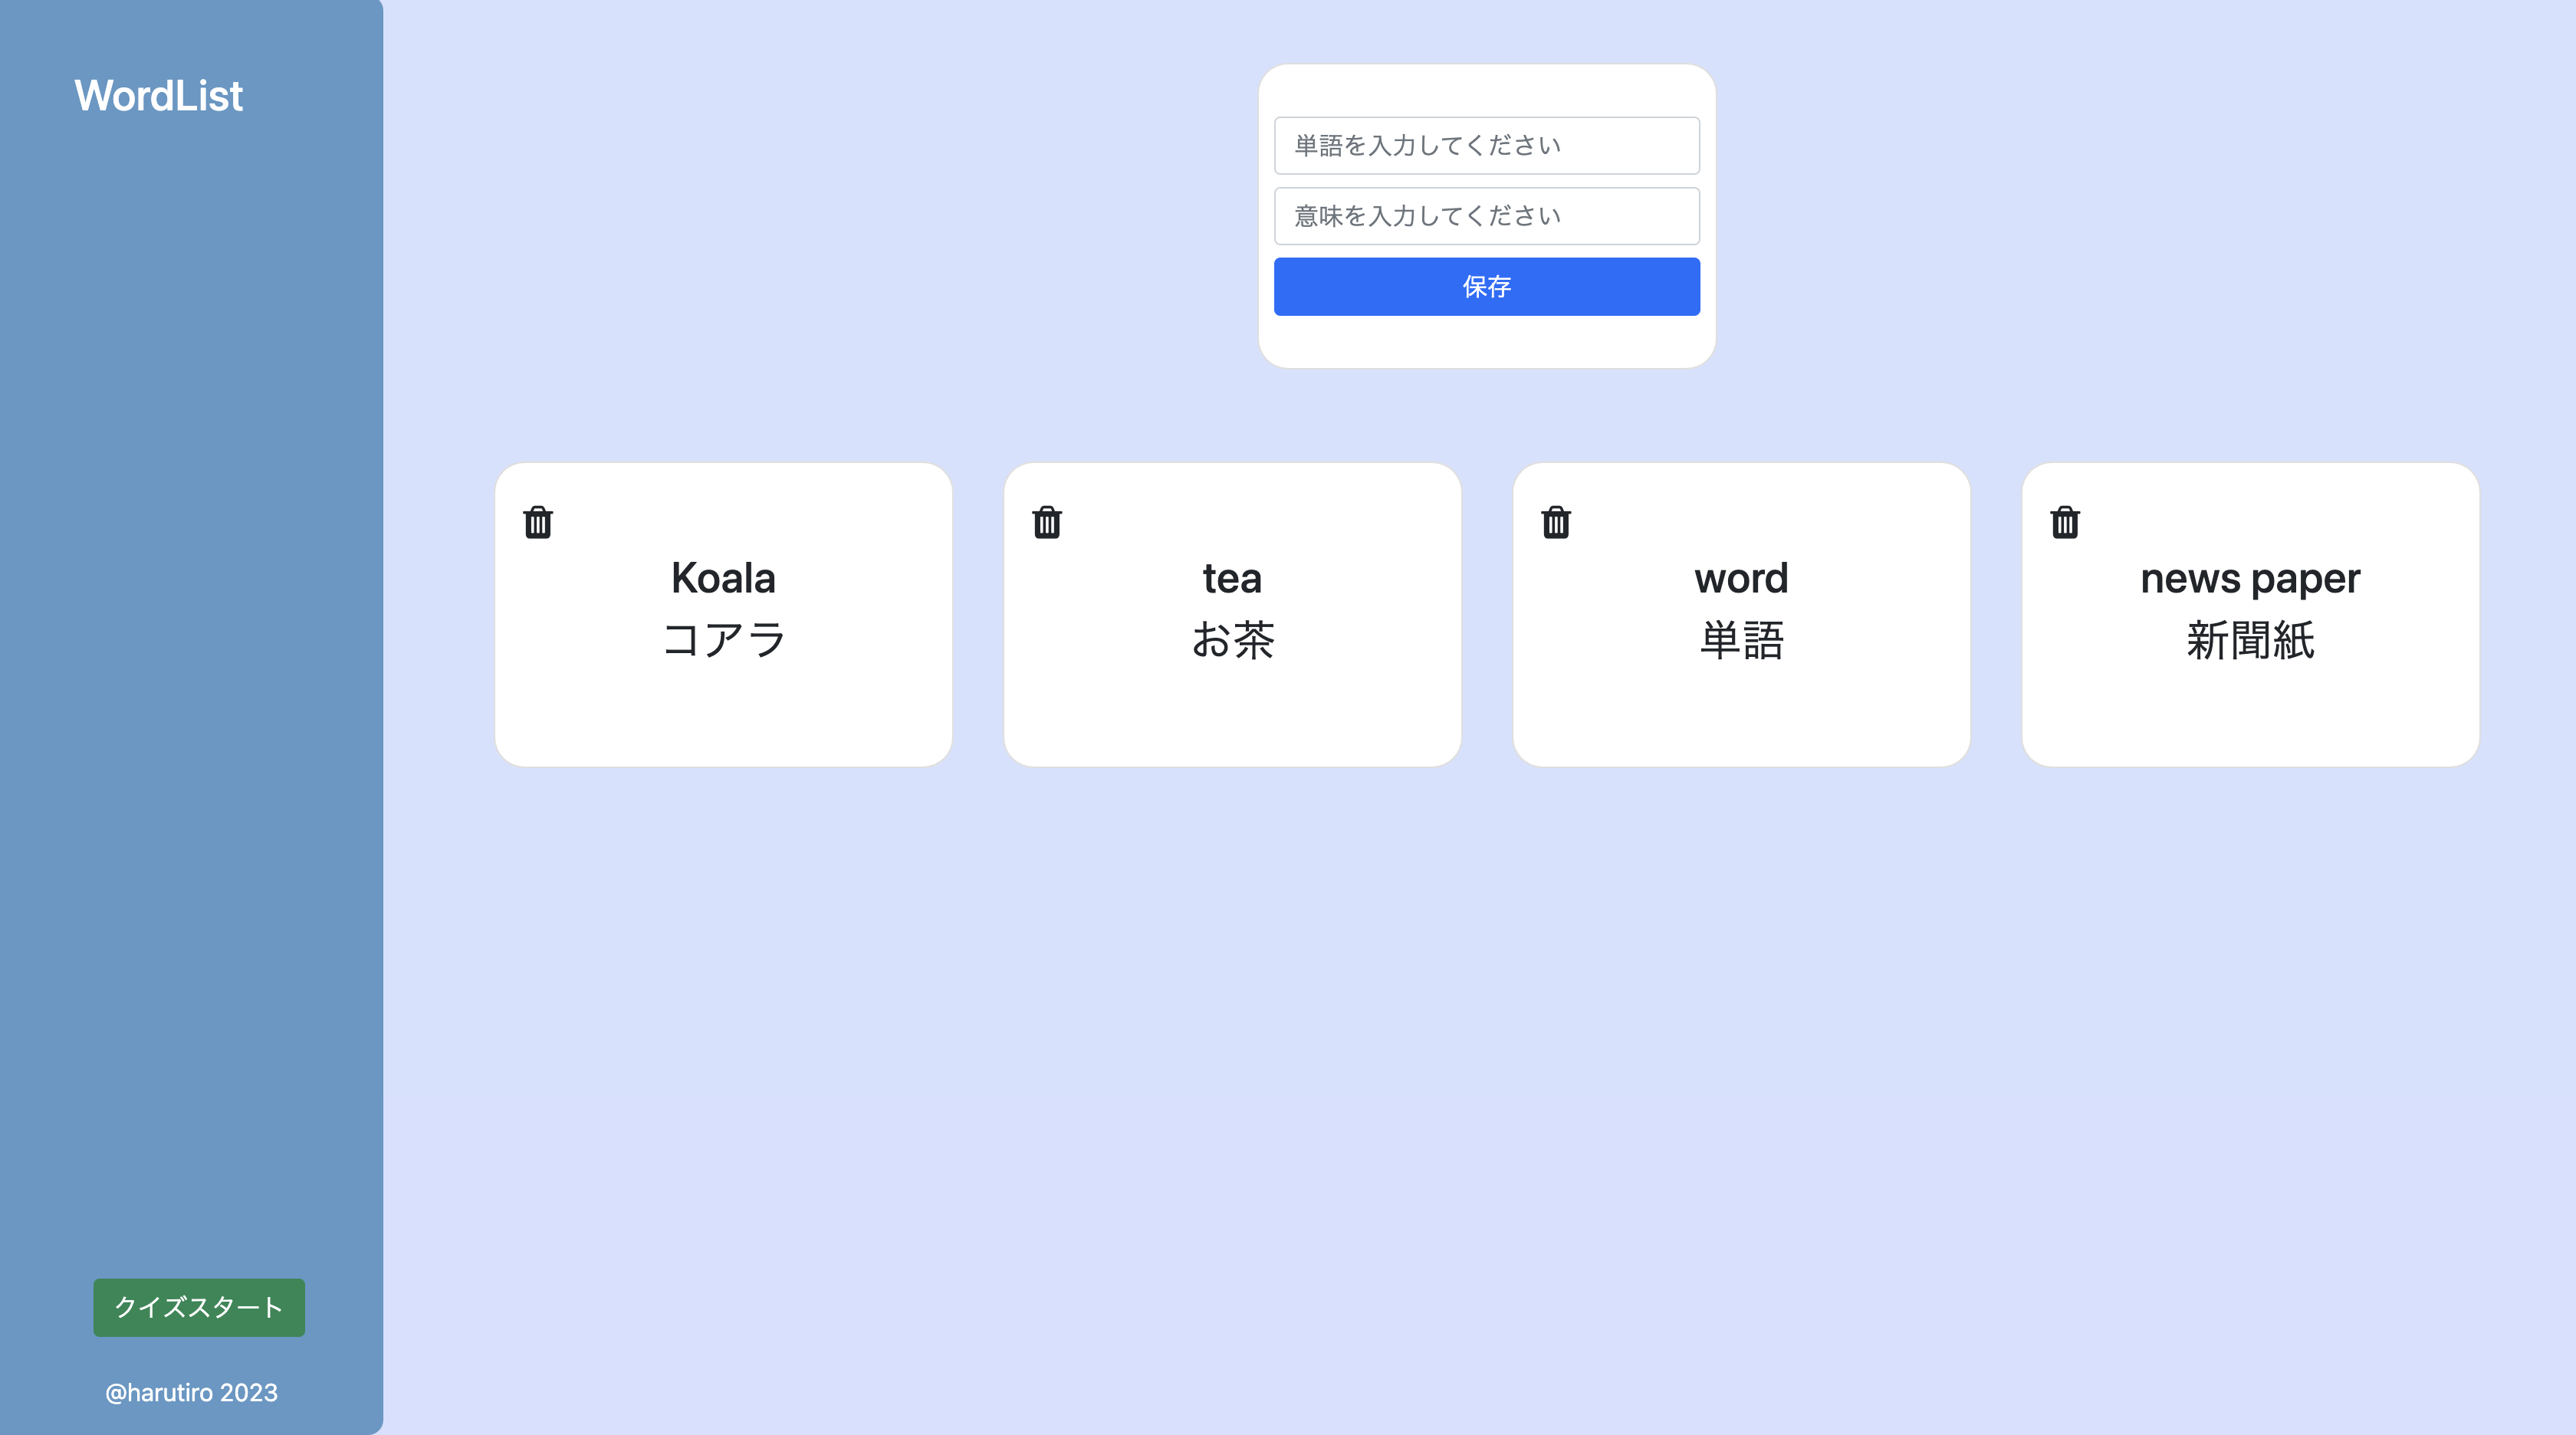
\includegraphics[width=70mm]{./img/edit_screen.png}

        \end{center}
        \caption{編集画面}
        \label{fig:edit_screen}
    \end{minipage}
    \begin{minipage}{0.5\hsize}
        \begin{center}
            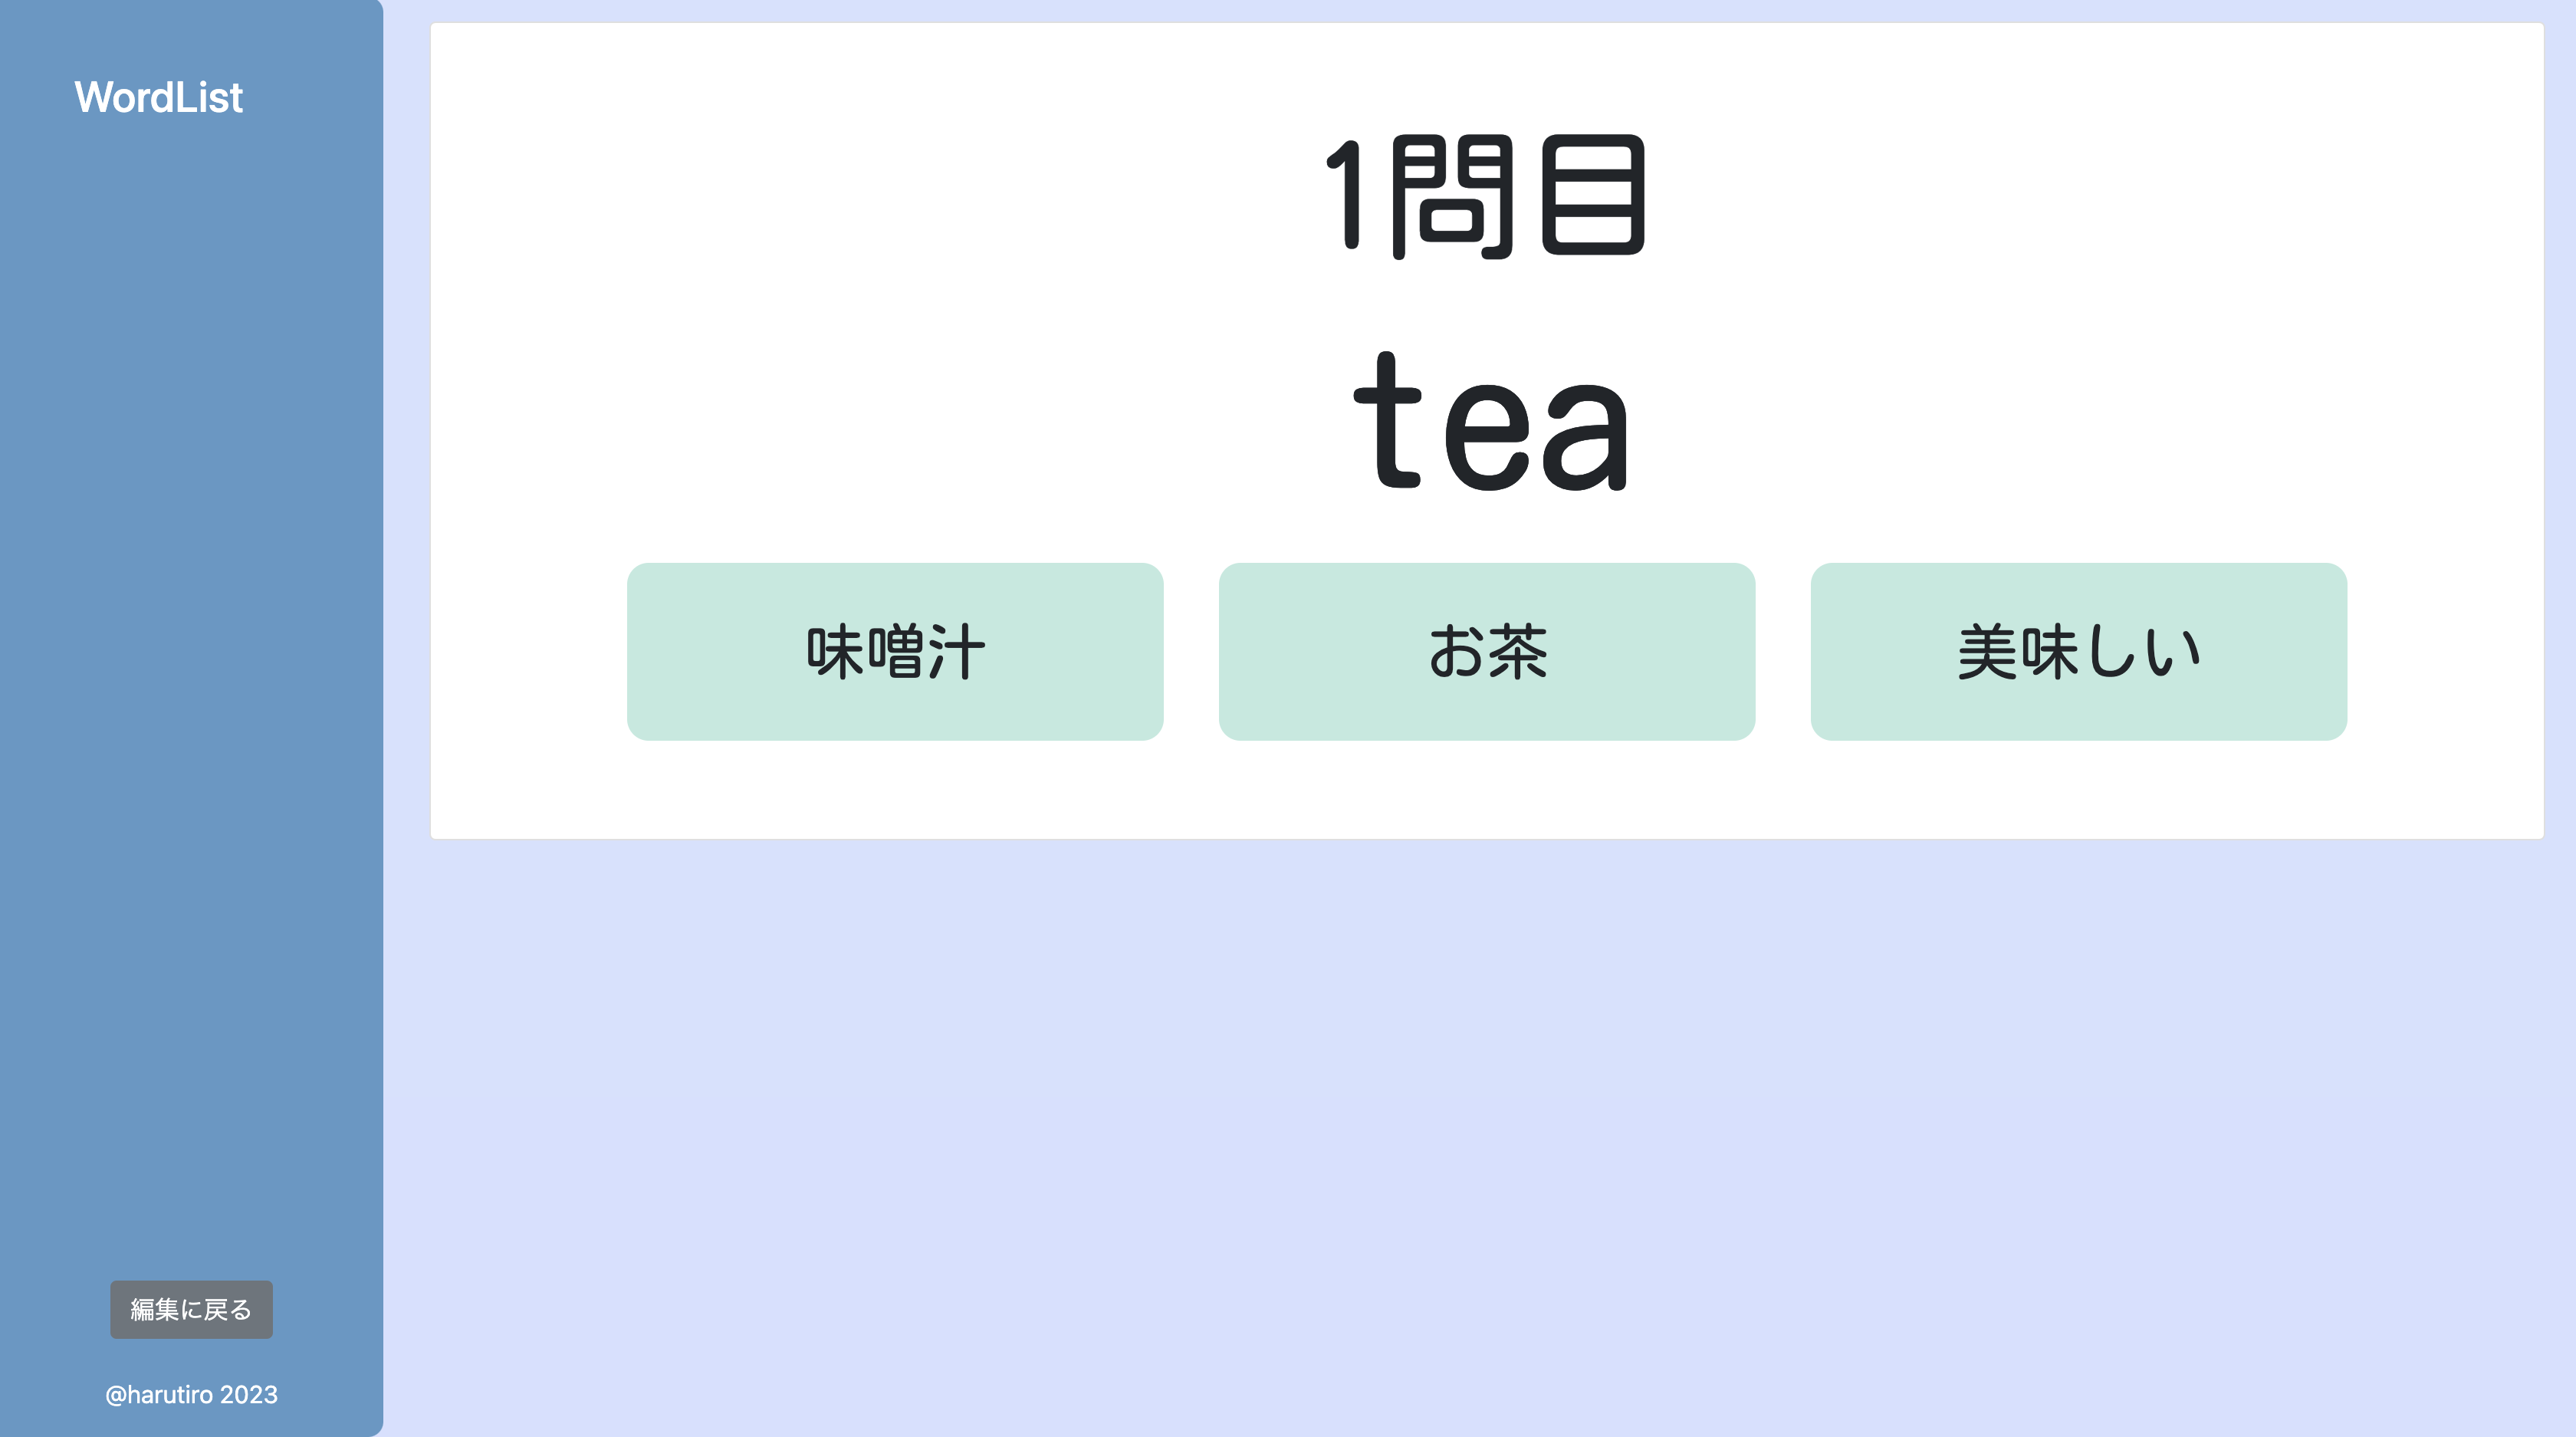
\includegraphics[width=70mm]{./img/quiz_screen.png}
        \end{center}
        \caption{クイズ画面}
        \label{fig:quiz_screen}
    \end{minipage}
\end{figure}

\subsection{編集画面}
編集画面では、単語とその意味を登録することができる。
単語とその意味を登録すると、クイズの自動生成ができるかどうかを判定する。

クイズの自動生成ができる単語は、今回APIで使用したWord2Vecの単語ベクトルに含まれている単語である。
Word2Vecとは、文章中の単語を数値ベクトルに変換してその意味を把握する自然言語処理の手法である。
数値ベクトルに変換を行っているため、演算処理をすることが可能で、cos類似度を用いることで単語の近侍度を求めることができる。
今回使用したWord2Vecのサンプルデータは日本語Wikipediaのサイトを用いているため、日本語以外の単語は対応していない場合が多い。
対応していない単語を用いると自動でクイズを生成することができないため、対応していない単語を登録されないようにエラー処理を行う。
クイズの自動生成ができない単語のエラー画面は図\ref{fig:quiz_error}に示す。
エラーを表示することにより、クイズの自動生成ができない単語を登録することを防ぎ、クイズの自動生成ができる単語のみを登録することができる。

覚えたい単語を登録したら、クイズ画面に移動することができる。
左下の緑のボタン「クイズスタート」を押し、クイズ画面に移動する。

%画像を出力する
\begin{figure}[htbp]
    \begin{center}
        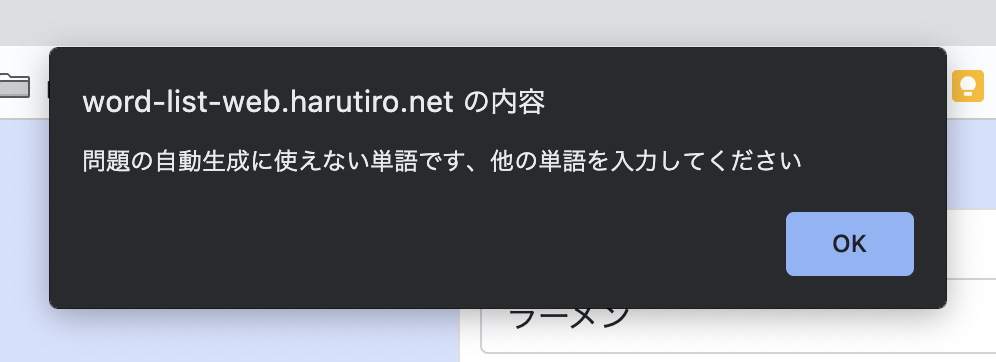
\includegraphics[width=70mm]{./img/error_popup.png}
    \end{center}
    \caption{クイズの自動生成ができない単語のエラー画面}
    \label{fig:quiz_error}
\end{figure}



\subsection{クイズ画面}
クイズ画面では、単語クイズを自動生成して楽しみながら覚えることができる。
クイズは3択クイズで、単語の意味を選択することができる。
クイズの自動生成は、Word2Vecの単語ベクトルを用いて行う。
正解の単語の意味に近い単語を50件取得し、その単語の中から二種類選択肢として表示する。
クイズの選択画面は図\ref{fig:quiz}に示す。

クイズは、回答をすると正誤に合わせた効果音を流すようにし、ユーザーエクスペリエンスを高めるように設計を行なった。
最後のクイズが終ると、クイズが終了したことをアナウンスする。
クイズの終了画面は図\ref{fig:quiz_end}に示す。



\begin{figure}[htbp]
    \begin{center}
        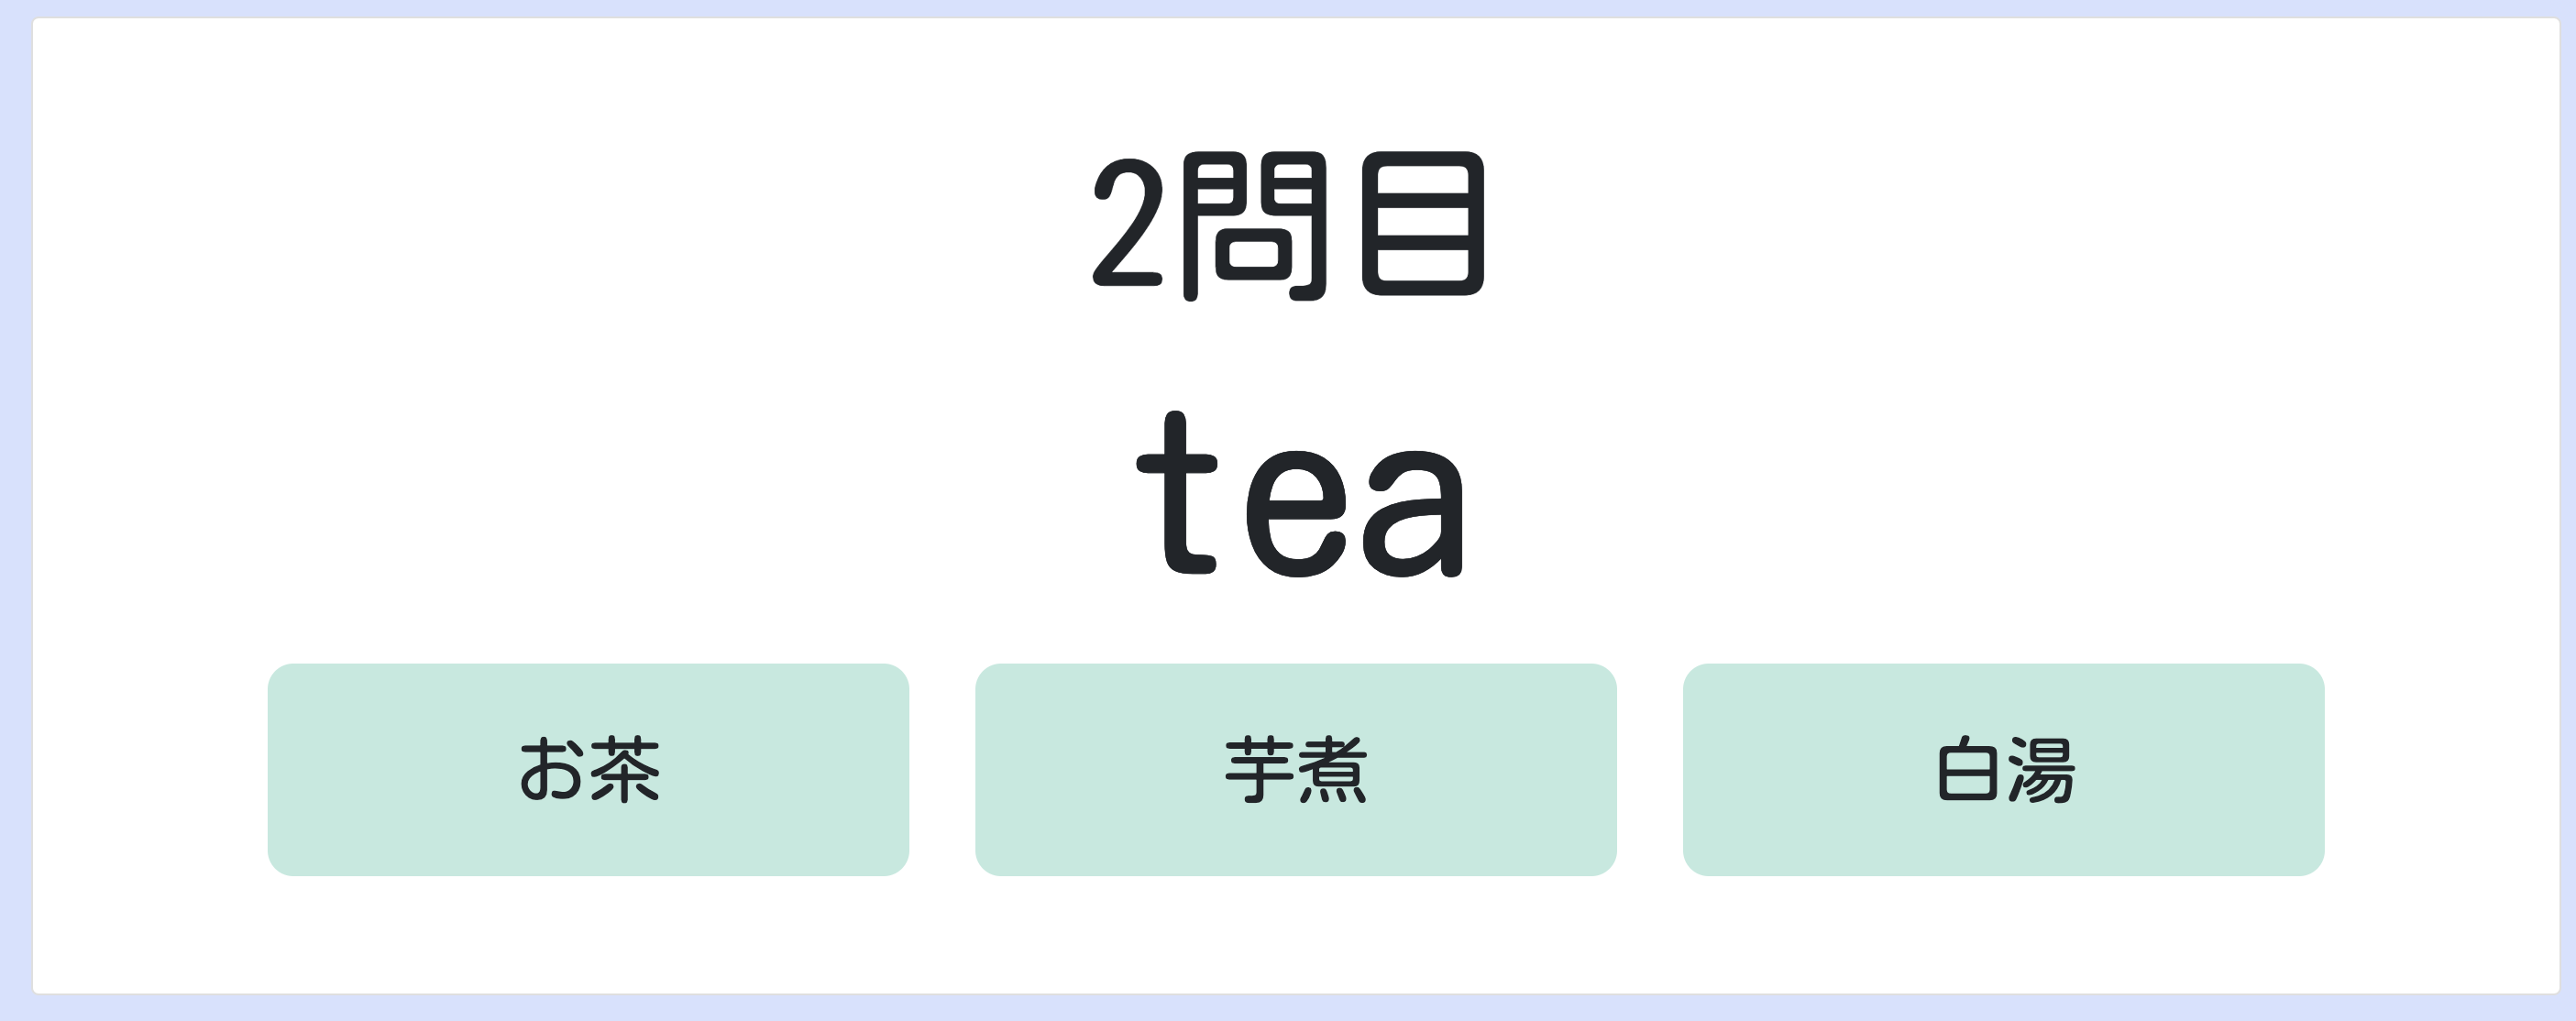
\includegraphics[width=70mm]{./img/question.png}
    \end{center}
    \caption{クイズの選択画面}
    \label{fig:quiz}
\end{figure}


\begin{figure}[htbp]
    \begin{center}
        
\includegraphics[width=70mm]{./img/question_end.png}
    \end{center}
    \caption{クイズの終了画面}
    \label{fig:quiz_end}
\end{figure}



\section{目的}
このアプリは、単語を覚えるのに面白みを持たせることで、単語を覚える時間を短縮することを目的としている。
そのため、単語を覚えるのに面白みを持たせるために、単語をクイズ形式にした。
そして、クイズを作成する時に、自分ですべての問題を作るというのは大変である。
そこで、単語の意味を入力するだけで、クイズを自動生成することができるようにした。
クイズの自動生成にはWord2Vecを用いることで、単語の意味を入力するだけで、単語の意味に近い単語を取得することができ、簡単にクイズを作成することができる。

機能面は、単語を登録し、クイズをするという中核をなす部分は完成している。
エラー処理なども行うことで、ユーザーがエクスペリエンスを上げることに成功し、満足のいくアプリケーションを作成することができた。
しかし、きめ細かい機能を追加することができなかったので、次の節では改善点を述べていく。


\subsection{改善点}
今後の改善点として、以下のようなものがある。
様々な単語を登録することで、様々なジャンルの単語が乱立してしまい覚えたい単語以外の単語もクイズに出てきてしまう問題点がある。
この問題点を解決するために、単語を登録する際に、単語のジャンルを登録することができるようにする。
単語のジャンルを登録することで、単語のジャンルを指定してクイズを出題することができる。

次に、Word2Vecの単語ベクトルを用いてクイズを自動生成しているため、単語ベクトルにない言葉はクイズに出題できない。
今回はWikipediaの記事をサンプルとして使用しているため、日本語以外の言語は単語ベクトルにあまり含まれていない。
この問題点を解決するために、英語版のWikipediaをサンプルとして使用することで、単語ベクトルに含まれていない単語もクイズに出題することができる。
また、中国語やフランス語にも対応させるため、世界各国のサンプルデータを取得することで、単語ベクトルに含まれていない単語もクイズに出題することができる。

\section{付録}

\subsection{API通信部分}

今回Word2Vecと通信を行うために、axiosを用いてAPI通信を行なった。
axiosを用いるメリットとして、使いやすく軽量である点、自動的なJSONデータ変換を行う点、
Promise APIにサポートしている点などがあるため本プログラムに採用した。
axiosを使用しているコードは図\ref{fig:axios}に示す。


\begin{figure}[htbp]
    \begin{center}
        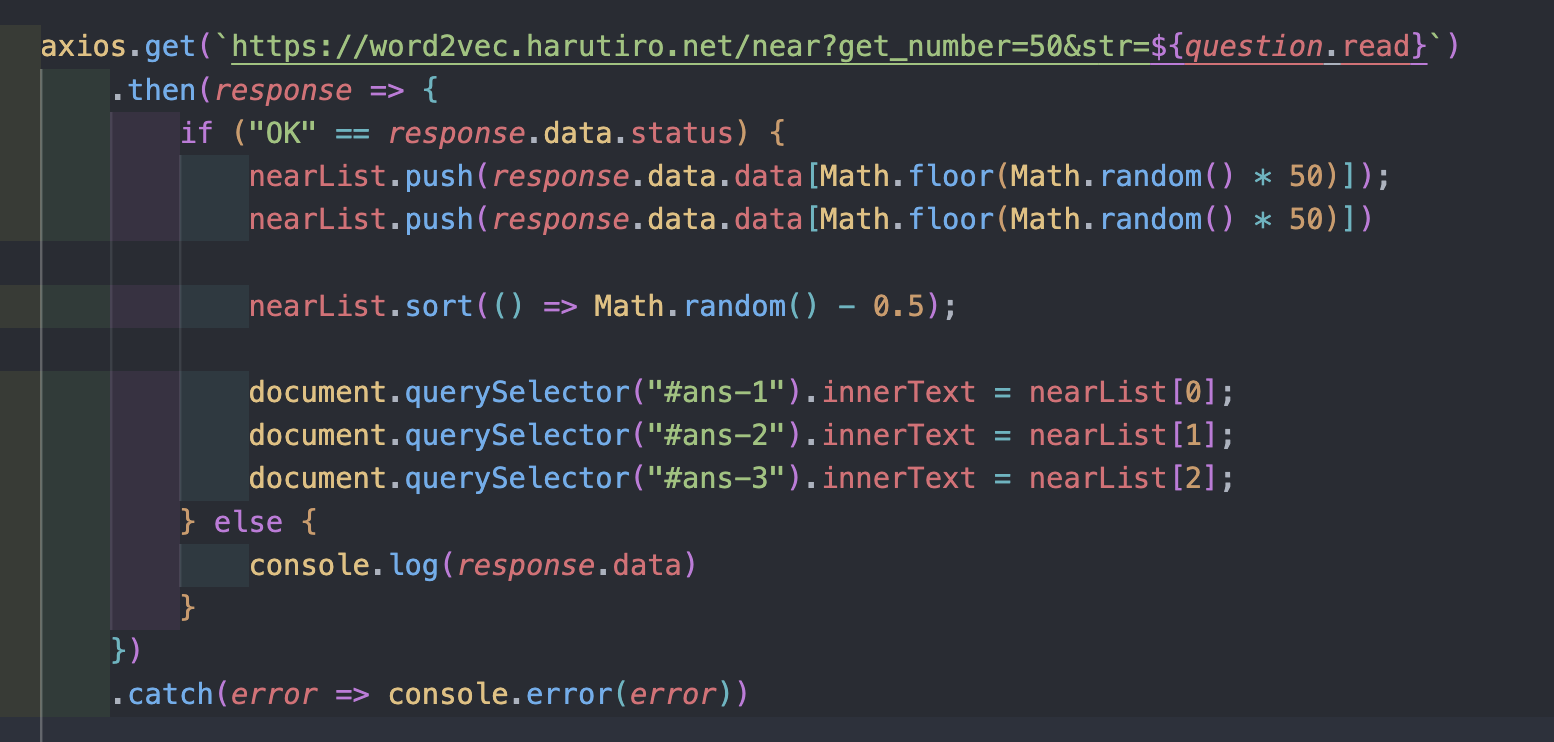
\includegraphics[width=100mm]{./img/axios.png}
    \end{center}
    \caption{axiosを使用しているコード}
    \label{fig:axios}
\end{figure}



\subsection{データクラスについて}

今後コードを更新するにあたり、わかりやすいソースコードを書く必要がある。
ソースコードをわかりやすく書くためには、明示的にデータを定義する必要がある。
そのため、データクラスを擬似的に定義を行い、ソースコードの可読性を高めた。
図\ref{fig:model},\ref{fig:new_word}は、データクラスの定義部分と使用部分を示している。


\begin{figure}[htbp]
    \begin{center}
        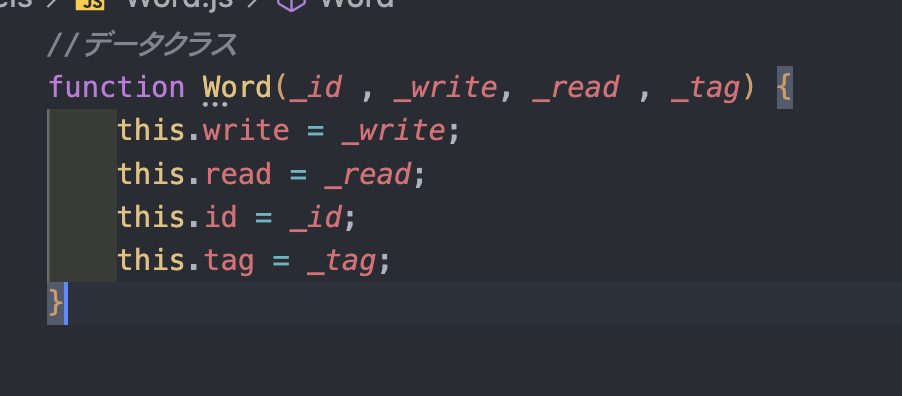
\includegraphics[width=100mm]{./img/model.png}
    \end{center}
    \caption{データクラスの定義部分}
    \label{fig:model}
\end{figure}

\begin{figure}[htbp]
    \begin{center}
        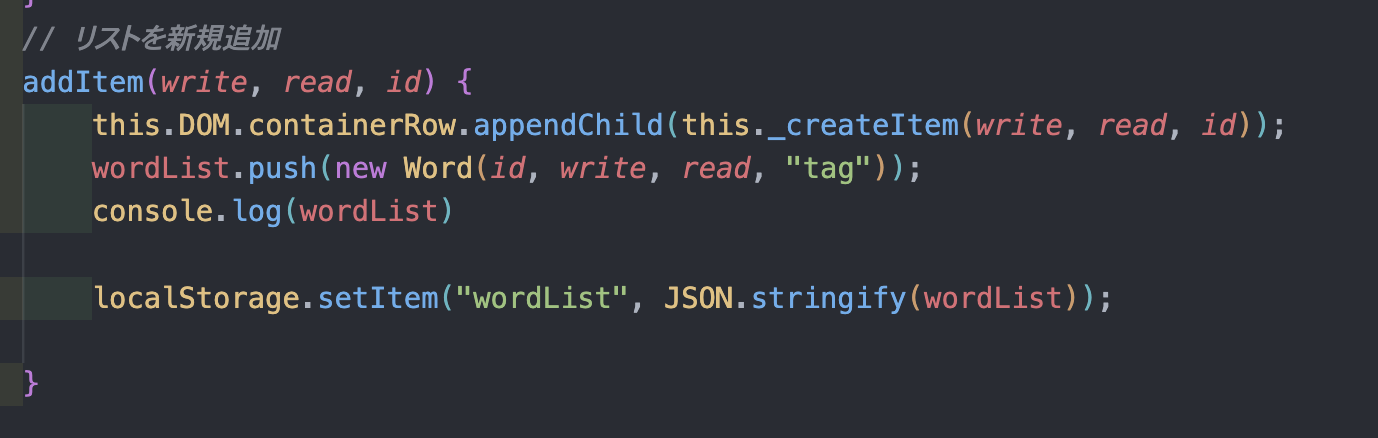
\includegraphics[width=100mm]{./img/new_word.png}
    \end{center}
    \caption{データクラスの使用部分}
    \label{fig:new_word}
\end{figure}

\subsection{デプロイについて}
今回のシステムは、GithubのPagesを用いてデプロイを行なった。
GithubのPagesを用いるメリットとして、無料で簡単にデプロイを行うことができる点、
Githubのリポジトリにあるソースコードをそのままデプロイすることができる点などがあるため本プログラムに採用した。
また、URLを独自ドメインに変更することで、より親しみやすいURLに変更することができる。

下記URLからアクセスできる。
https://word-list-web.harutiro.net/


\subsection{cssについて}
今回、わかりやすいUIを作成するため、クラウドベースのユーザーインターフェイスデザインツールである、Figmaを用いてUI設計を行なった。
UI設計をするにあたり、マテリアルデザインに準拠をしどんなユーザーにも直感的に操作ができるようなデザインを心がけた。

統一されたデザインを作成するため、bootstrapを用いて開発を行なった。
classを使用するだけで簡単にcssを記載することができるためとても便利である。
図\ref{fig:ptag}は、bootstrapを用いてcssを記載している例である。

\begin{figure}[htbp]
    \begin{center}
        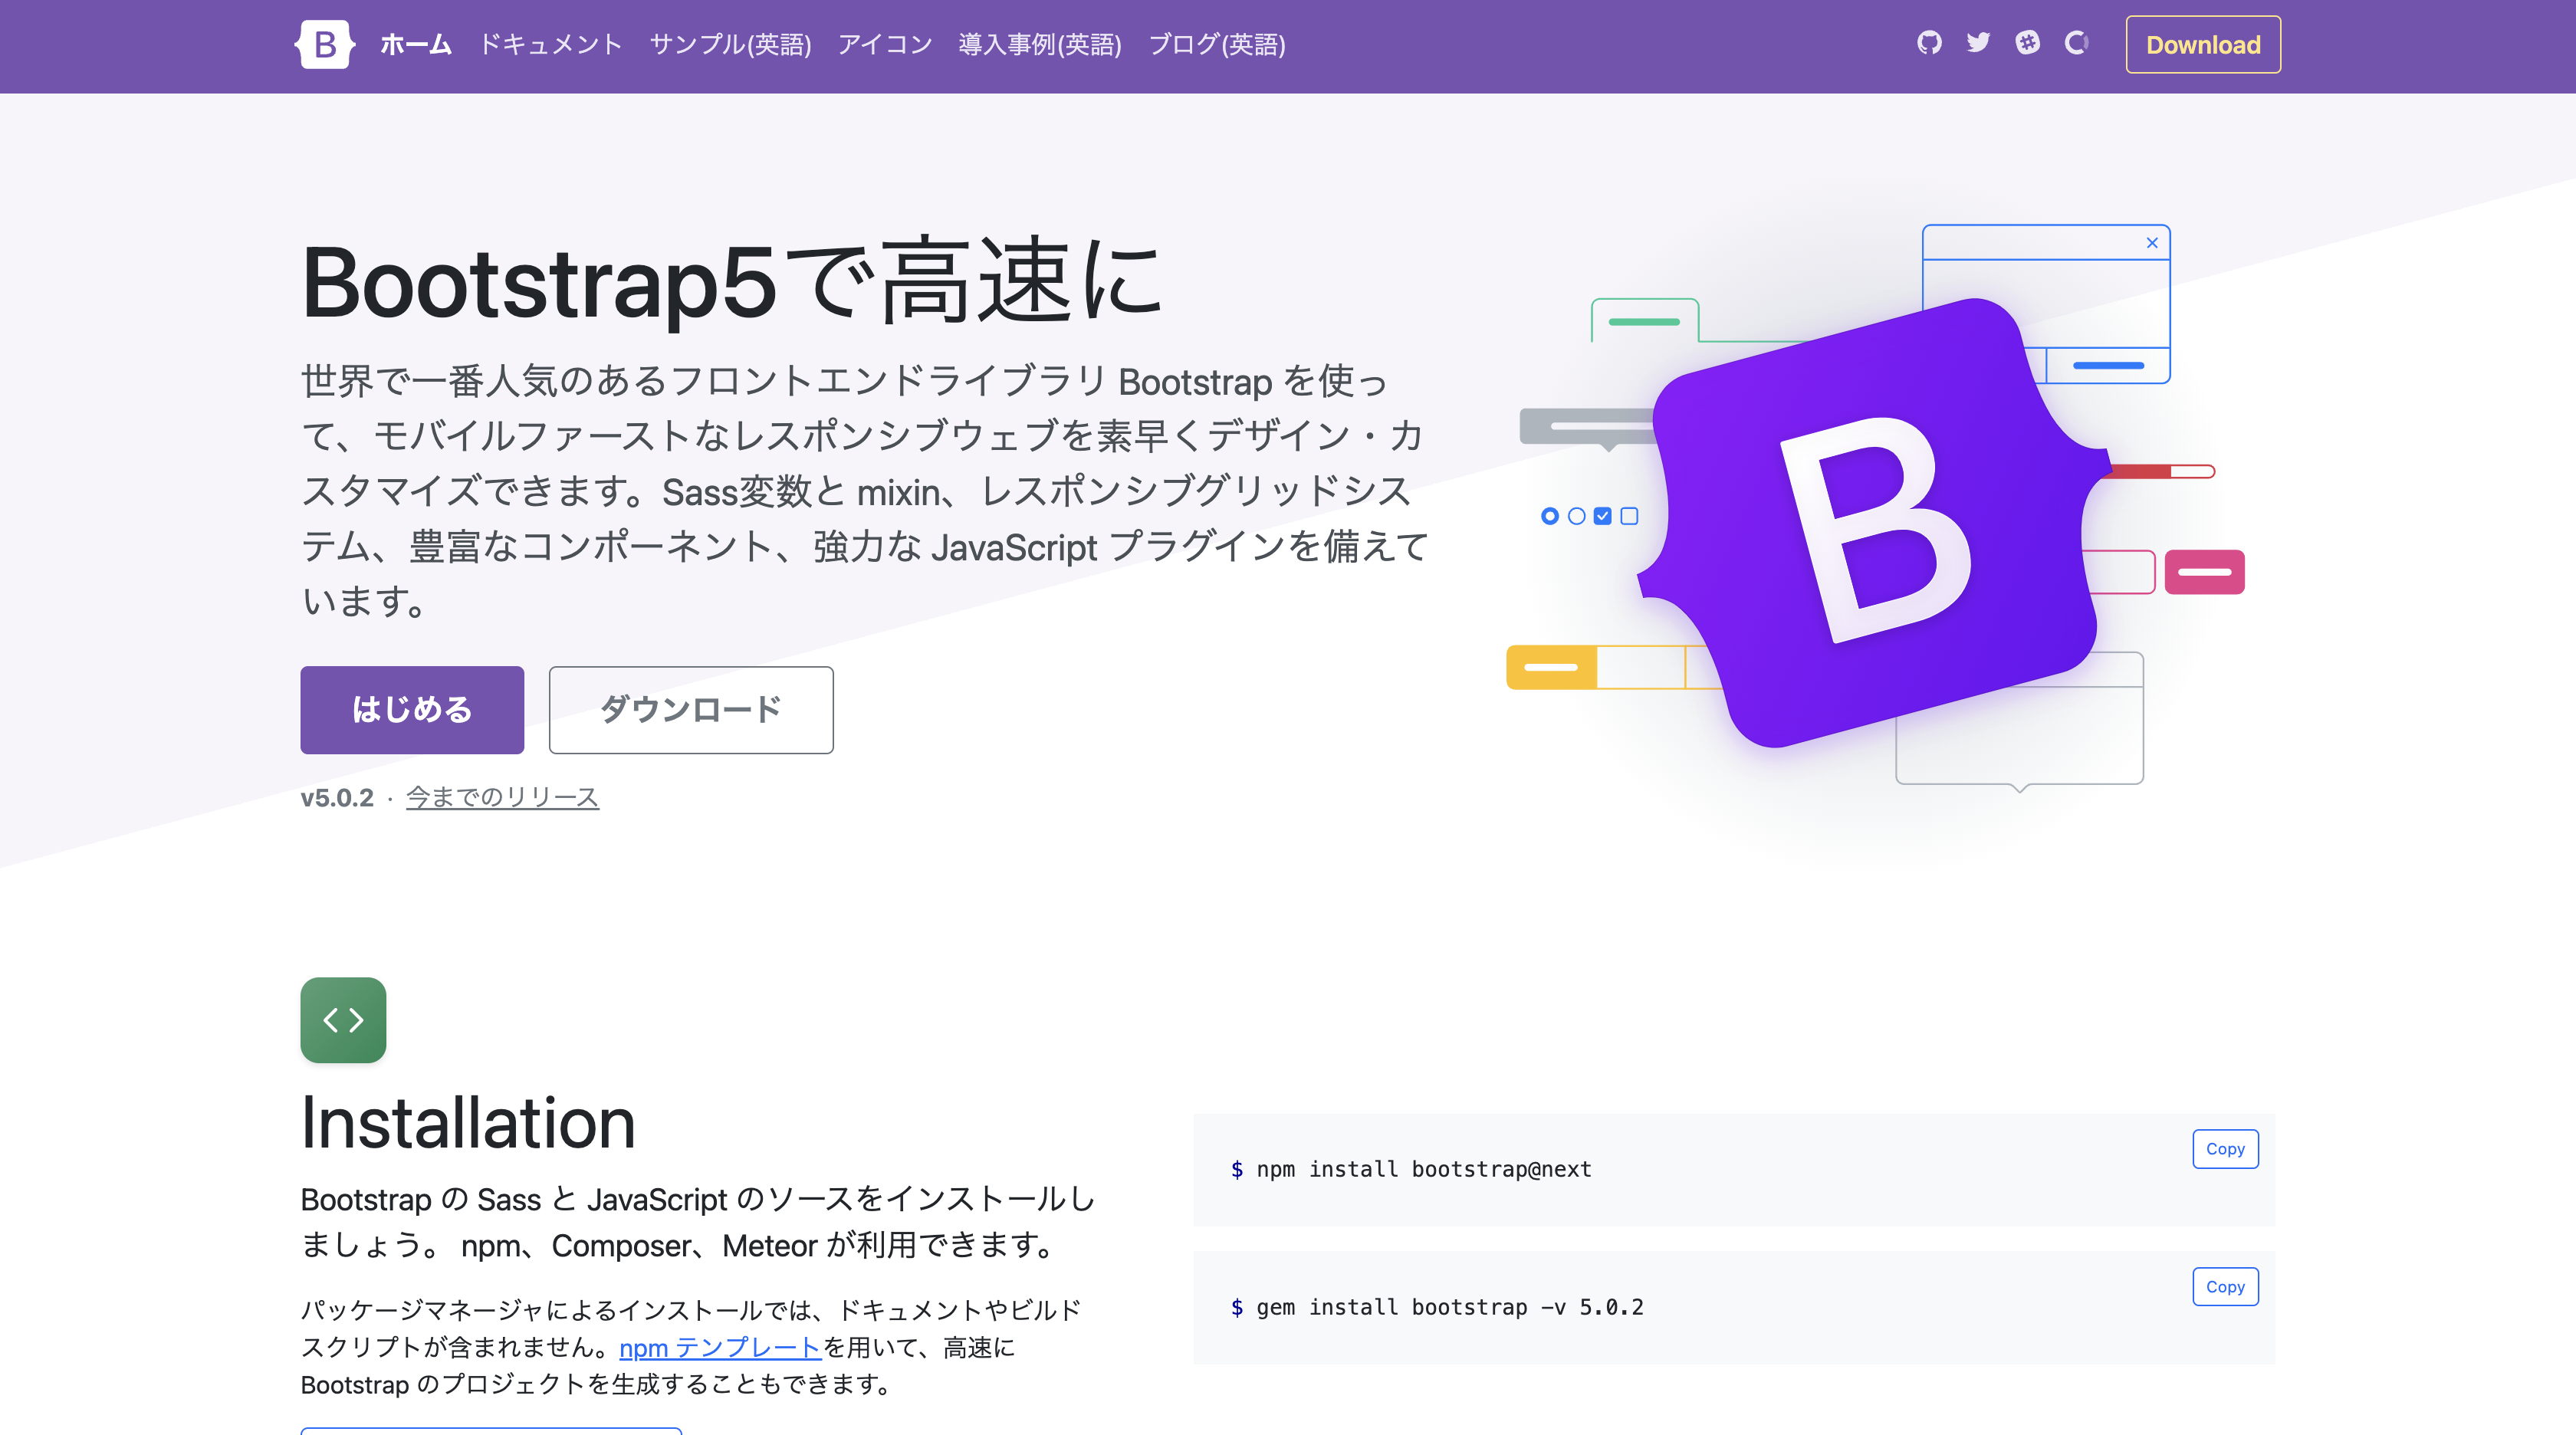
\includegraphics[width=100mm]{./img/bootstrap.png}
    \end{center}
    \caption{Bootstrapの公式ページ}
\end{figure}

\begin{figure}[htbp]
    \begin{center}
        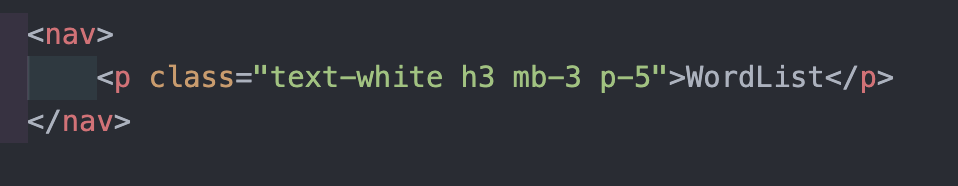
\includegraphics[width=100mm]{./img/ptag.png}
    \end{center}
    \caption{Bootstrapを用いてcssを記載している例}
    \label{fig:ptag}
\end{figure}



\subsection{faviconについて}
faviconは、ブラウザのタブに表示されるアイコンである。
今回は、faviconを作成するために、Figmaを使用した。
Figmaを使用するメリットとして、簡単にアイコンを作成することができる点、
アイコンを作成する際に、デザインを統一することができる点などがあるため本プログラムに採用した。
図\ref{fig:favicon}は、Figmaを使用して作成したfaviconである。

\begin{figure}[htbp]
    \begin{center}
        
\includegraphics[width=40mm]{./img/favicon.png}
    \end{center}
    \caption{Figmaを使用して作成したfavicon}
    \label{fig:favicon}
\end{figure}







\end{document}
